\documentclass[journal,comsoc]{IEEEtran}
%\documentclass[conference]{IEEEtran}
%\documentclass[conference]{ieeeconf}  
%\documentclass[a4paper,10pt,conference]{ieeeconf}                                                              
\IEEEoverridecommandlockouts                                                                                           
%\overrideIEEEmargins
%% command later in the file to balance the column lengths
%%\addtolength 
\usepackage {cite}
\usepackage {amsmath,amssymb,amsfonts}
%\usepackage{amsmath,amssymb,amsfonts,amsthm,mathtools,latexsym} 
\usepackage {algorithmic}
\usepackage {graphicx}
\usepackage	{textcomp}
\usepackage	{xcolor}
\usepackage	[spanish,english]{babel}
%\usepackage[T1]{fontenc}
\usepackage	[utf8x]{inputenc}
\usepackage	{threeparttable}
\usepackage	{multirow}
\usepackage {lscape}
\usepackage {float}
\usepackage	{caption}
\usepackage	{subcaption}
%\usepackage{graphics} 	% for pdf, bitmapped graphics files
\usepackage {epsfig} 	% for postscript graphics files
%\usepackage{mathptmx} 	% assumes new font selection scheme installed
%\usepackage{times} 	% assumes new font selection scheme installed
%\usepackage{stackrel}
%\usepackage{lastpage}
%\usepackage{subfigure}
%\usepackage{hyperref}
\def\BibTeX{
{\rm B\kern-.05em{\sc i\kern-.025em b}\kern-.08em
T\kern-.1667em\lower.7ex\hbox{E}\kern-.125emX}
}
	
	
%%%%%%%%
% INICIO
%%%%%%%%
\begin{document}
\title{
\huge \bf VLSI Implementation of a Pipelined 128 points 4-Parallel radix-$\mathbf{2^3}$ FFT Architecture via Folding Transformation
}
\author{
James J. W. Kunst   \\{\tt\small jjwk89@gmail.com}		\\
Kevin H. Viglianco	\\{\tt\small kevinvig7@gmail.com}	\\ 
Daniel R. Garcia	\\{\tt\small dani6rg@gmail.com}		\\
[0.5cm]
{\large \bf Digital Signal Processing in Very Large Scale Integration Systems}\\
[0.5cm]
Autumn 2019\\
[0.5cm]
Dr. Keshab K. Parhi	\\
Dr. Ariel L. Pola	\\
[0.5cm]
Universidad Nacional de Córdoba - FCEFyN\\
Av.Vélez Sársfield 1611, X5016GCA, C\'ordoba, Argentina\\
[0.5cm]
Fundación FULGOR\\
Ernesto Romagosa 518, Colinas V. Sarsfield, X5016GQN, Córdoba, Argentina         
}
\maketitle


%%%%%%%%%%
% Abstract
%%%%%%%%%%
\begin{abstract} - \bf In this work we present a develop and VLSI implementation of a 4-parallel pipelined architecture for the complex fast Fourier transform (CFFT) based on the radix-$\bf 2^3$ algorithm with 128 points using folding transformation and register minimization techniques. In addition, we are going to generate different synthesis levels from the hardware language description (HDL) with the purpose of obtaining a suitable performance on speed and area. %A comparison is drawn between the proposed designs and the original architecture.
\end{abstract}
%%%%%%%%%
% Seccion
%%%%%%%%%
\section{INTRODUCTION}
The Fast Fourier Transform (FFT) is widely used in different applications' fields, particularly, it is used in algorithms that involves apply digital signal processing, e.g., calculate the Discrete Fourier Transform (DFT) efficiently, that is useful because in some applications is most convenient to work in frequency domain than time domain. Nowadays is common utilize the algorithm of FFT for real time applications and parallel-pipelined hardware architecture give us the opportunity to work at hight throughput rates.

There are two main types of pipelined FFT architectures \cite{shousheng_he_designing_1998}. On the one hand, feedback architectures (FB) which can be divided into Single-path Delay Feedback (SDF) and Multi-path Delay Feedback (MDF), theses methods take out samples from each butterflies stages and feed back to the registers or memories at the same stage. On the other hand, feedforward architectures such as Multi-Path Delay Commutator (MDC) where the main difference with the feedback architectures is that SDF transfer data samples from one stage to other stage serially, instead of that the MDC architecture transfer more than one sample per clock cycle and do not have feedback loops.

This work focuses on the design of 4-parallel pipelined architecture radix-$2^3$ 128-points for Complex FFT-DIF (Decimation in frequency). First, we will obtain the equations that correspond to Bufterfly structure of \textit{radix}-$2^3$ FFT-DIF for 8 points. After that, we apply these idea to design a 2-parallel pipelined architecture radix-$2^3$ 16-points FFT via folding transformation and find the appropriates rotators (\textit{twiddles}) for each stage and clock cycle over the chain of butterflies on a feedforward architecture MDC. Second, we elaborate a float-point simulator which will process a summation of two cosine signals with different frequencies. Later, for the input and output of each stage of DFT, we quantized all operations such as adders and multipliers to get a fixed-point model. In this way, we can compare both models verifying the Signal to quantization noise ratio (SQNR) between fixed and float models.

Furthermore, we take the fixed-point model to elaborate our Synthesizable Verilog code HDL and verify the DFT functionality in each stage of the architecture. In addition to this, we generates power-area-timing report with different optimizations such as varying pipelining levels and canonical signed digit (CSD).
%%%%%%%%%
% Seccion
%%%%%%%%%
\section{DESIGN OF FFT ARCHITECTURE VIA FOLDING}
%T h e d evelop m en t o f com p utationally efficient algorithm s for the D F T is m ade pos­
%sible if w e adopt a divide-and-conquer approach. T his approach is based on the
%d ecom p osition o f an Af-point D F T in to su ccessively sm aller D F T s. T his basic ap­
%proach leads to a fam ily o f com putationally efficient algorithm s k n ow n collectively
%as FFT algorithm s.

%A n o th e r im portant radix-2 FFT algorithm , called th e decim ation -in-freq u en cy
%algorithm , is o b tain ed by using the divide-and-conquer approach described in S ec­
%tion 6.1.2 w ith th e ch oice o f M = 2 and L = N f l . T his ch oice o f param eters
%im plies a colu m n-w ise storage o f the input data seq u en ce. T o d erive the algo­
%rithm, w e begin by splitting the D F T form ula in to tw o sum m ations, o n e o f which
%in v o lv es the sum over the first N t 2 data p oin ts and th e secon d sum in volves the
%last N I 2 data points.
In this section, we illustrate the folding transformation method to derive a 16-point DIF FFT 4-parallel architecture as an example and then, using the same method, we extend it to 128-point architecture. To do this, we will use the architecture proposed in \cite{ayinala_pipelined_2012}.
%%%%%%%%%%%%
% Subseccion
%%%%%%%%%%%%
\subsection{4-Parallel radix-$2^3$ 16-Points}
In Fig. \ref{fig:flowgraph_16}  we can see the flow graph of a 16-point DIF FFT radix-2. The graph is divided into four stages and each of them consist of a set of butterflies and multipliers. The twiddle factor in between the stages indicates a multiplication by $W^k_N$, where $W_N$ denotes the \textit{N}th root of unity, with its exponent evaluated modulo N. This can be represented as a DFG as shown in Fig. \ref{fig:dfg_16} where the nodes represents the butterfly computations of the radix-2 FFT algorithm. 

\begin{figure}[htbp]
\centering
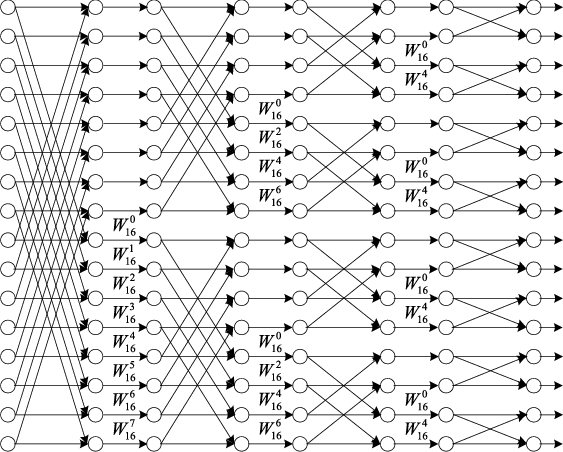
\includegraphics[width=\linewidth]{Diagramas/fft16.png}%
\caption{Flow graph of a radix-2 16-point DIF FFT.}
\label{fig:flowgraph_16}
\end{figure}

\begin{figure}[htbp]%[ht]
\centering
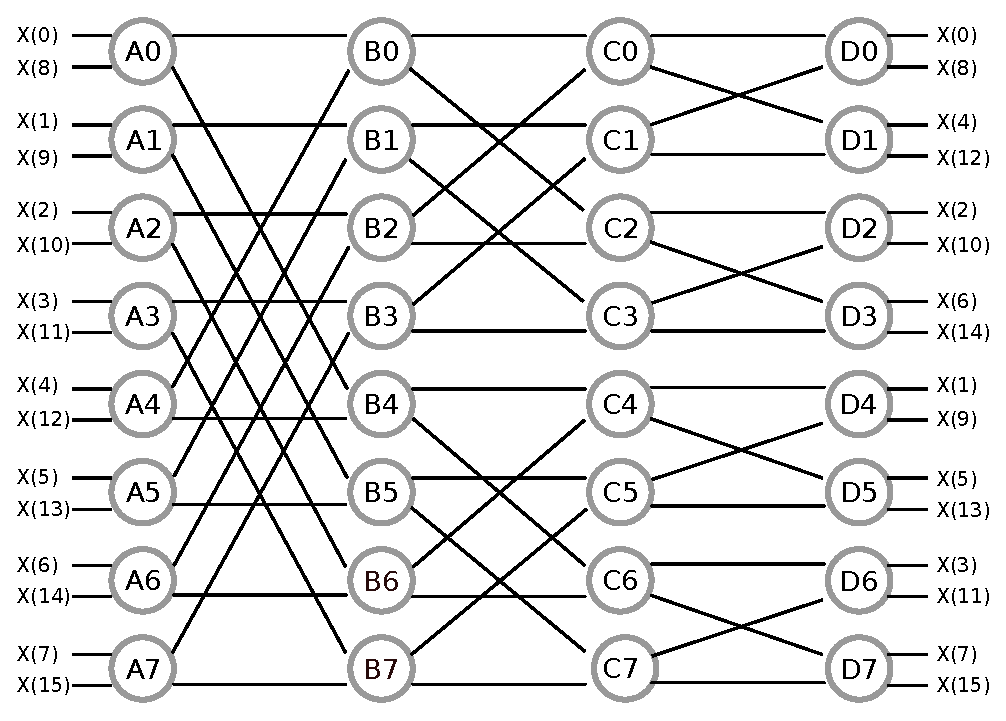
\includegraphics[width=\linewidth]{Diagramas/Butter16.eps}
\caption{Data Flow graph (DFG) of a radix-2 16-point DIF FFT.}
\label{fig:dfg_16}
\end{figure}

The folding transformation is used on the DFG in to derive a pipelined architecture. To do this we need a folding set, which is an ordered set of operations executed by the same functional unit. Each folding set contains K entries, where K is called the folding factor. The operation in the \textit{j}th position within the folding set (where goes from 0 to K-1) is executed by the functional unit during the time partition. The term is called the folding order.

First we need to derive the folding equations, to do this consider an edge $e$ connecting the nodes \textit{U} and \textit{V} with $w(e)$ delays. Let the executions of the \textit{l}th iteration of the nodes \textit{U} and \textit{V} be scheduled at the time units $Kl+u$ and $Kl+v$ respectively, where $u$ and $v$ are the folding orders of the nodes \textit{U} and \textit{V}, respectively. The folding equation for the edge $e$ is:

\begin{equation}
    D_F(U \to V) = Kw(e)-P_U+v-u
\end{equation}

where $P_U$ is the number of pipeline stages in the hardware unit which executes the node U.

Consider folding of the the DFG in Fig. \ref{fig:dfg_16} with the folding sets:

\begin{align*}
    A&= \{ A0,A2,A4,A6 \}  & A'&= \{ A1,A3,A5,A7 \} \\
    B&=\{ B1,B3,B0,B2 \}  &B'&=\{ B5,B7,B4,B6 \} \\
    C&=\{ C2,C1,C3,C0 \}  &C'&=\{ C6,C5,C7,C4 \} \\ 
    D&=\{ D3,D0,D2,D1 \}  &D'&=\{ D7,D4,D6,D5 \} 
    \label{eq:foldingset_16}
\end{align*}

Assuming that the butterfly operations do not have any pipeline stages ($P_A=P_B=P_C=P_D=0$), the folding equations can be derived for all edges (see \ref{sec:appen:folding_eq}). For the folded system to be realizable, $D_F(U\to V)\geq0$ must hold for all the edges in the DFG. Retimming and/or pipeline can be applied to satisfy this property, if the DFG in Fig. \ref{fig:dfg_16} is pipelined/retimmed as shown in Fig. \ref{fig:dfg_16_ret} the system is realizable and the folded delays for the edges are given by \ref{sec:appen:folding_eq_ret}.

\begin{figure}[htbp]%[ht!]
\centering
 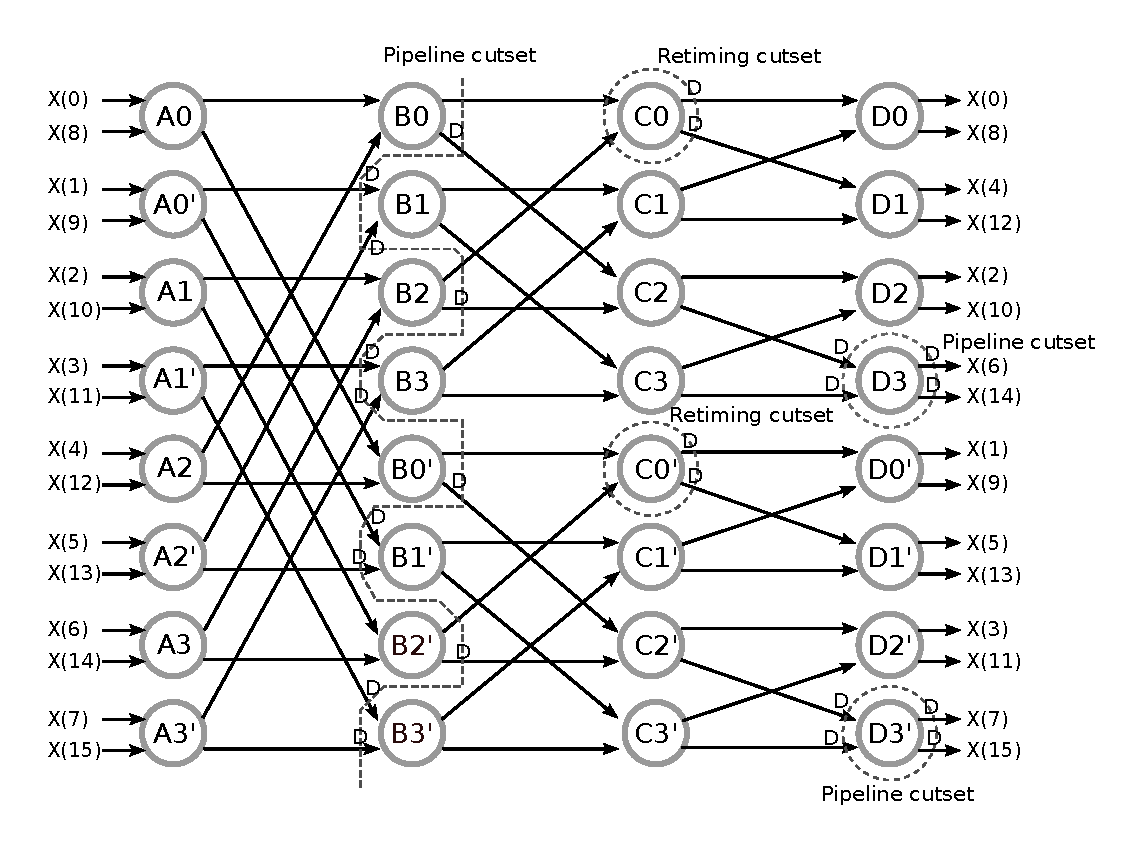
\includegraphics[width=\linewidth]{Diagramas/Butter16_pipe.eps}%
\caption{Data Flow graph (DFG) of a radix-2 16-point DIF FFT with retimming and pipeline.}
\label{fig:dfg_16_ret}
\end{figure}

We can see that the number of register required to implement the folding equations in \ref{sec:appen:folding_eq_ret} is 80. For minimize the number of registers we use the register minimization technique. 
If we let the output of node A1 be $y_{(0)}$ and $y_{(8)}$, applying this successively with the rest of the nodes A we can obtain the linear life time chart for this stage in Fig. \ref{fig:tab-life-a}. Applying this criteria to the rest of the stages we can obtain the life time chart \ref{fig:tab-life-b} and \ref{fig:tab-life-c} for the outputs of the nodes B and C respectively, we can see that the numbers of maximum registers in each stage are 8, 4 and 8 respectively. More information about this method can be found on \cite{pipeline_parhi_book}.

\begin{figure}[htbp]%[ht!]
\centering
 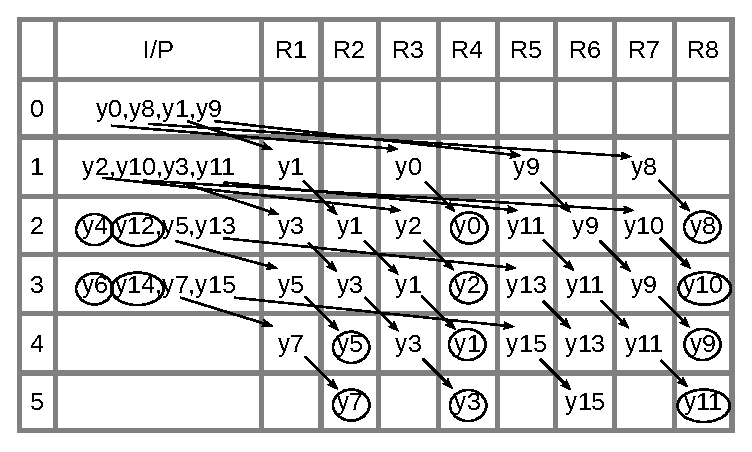
\includegraphics[width=\linewidth]{Diagramas/tab_life_a.eps}%
\caption{Linear lifetime chart for the variables $y_{(0)}, y_{(1)},...,y_{(15)}$ for a 16-point FFT architecture.}
\label{fig:tab-life-a}
\end{figure}

\begin{figure}[htbp]%[ht!]
\centering
 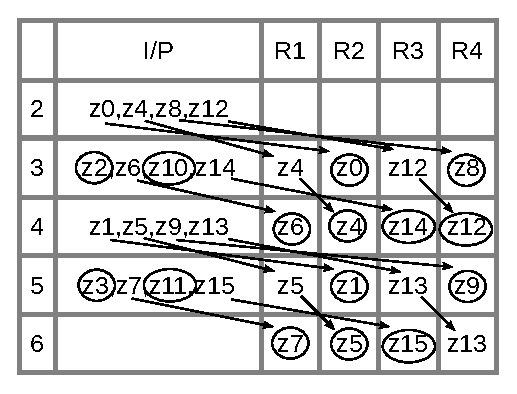
\includegraphics[width=0.7\linewidth]{Diagramas/tab_life_b.eps}%
\caption{Linear lifetime chart for the variables $z_{(0)}, z_{(1)},...,z_{(15)}$ for a 16-point FFT architecture.}
\label{fig:tab-life-b}
\end{figure}

\begin{figure}[htbp]%[ht!]
\centering
 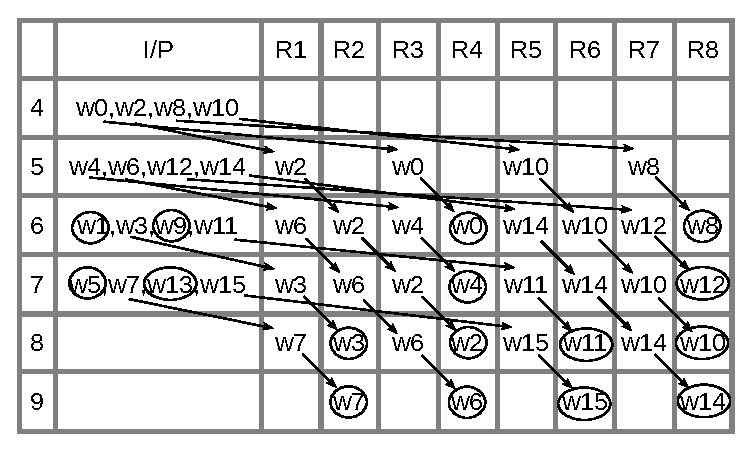
\includegraphics[width=0.8\linewidth]{Diagramas/tab_life_c.eps}%
\caption{Linear lifetime chart for the variables $w_{(0)}, w_{(1)},...,w_{(15)}$ for a 16-point FFT architecture.}
\label{fig:tab-life-c}
\end{figure}

The register allocation tables for each of lifetime charts are shown in Fig. \ref{fig:tab-aloc-a}, \ref{fig:tab-aloc-b} and \ref{fig:tab-aloc-c} respectively, we can implement the same equations in \ref{sec:appen:folding_eq_ret} using 20 registers with register minimization techniques. The folded architecture in Fig. \ref{fig:circ-folding-16} is synthesized using the folding equations and the register allocation tables, the method can be found in \cite{pipeline_parhi_book}. 

The inputs of each folding node are represented with a matrix where the values in the same column are data that flow in parallel and values in the same row
flow through the same path in consecutive clock cycles. The first two rows represents the inputs of the superior BF and the others two represents the input of the inferior BF. 
The same criteria is used for represent the constants of rotators, where each number $k$ of the matrix represent a multiplication by $W^k_N$.

As we can see in \ref{fig:circ-folding-16}, we suppose that the inputs and output are not ordered, to order these variables extra logic are needed, using more registers and multiplexers.

The different types of rotators used in Fig. \ref{fig:circ-folding-16} are shown in Fig. \ref{fig:rotators}, the description of each of them can be found below.

\begin{itemize}

\item Trivial rotator: They can be carried out by interchanging the real and imaginary components and/or changing the sign of the data.
\item Constant CSD rotator: They can be carried out by interchanging the real and imaginary components and/or a multiplication by a unique constant fractional number, in this case we will use a CSD multiplier to perform the area utilized.
\item General rotator: They can be carried out by interchanging the real and imaginary components and/or a multiplication by more than one constant fractional numbers, in this case we will use a general multiplier.

\end{itemize}

\begin{figure}[htbp]%[ht!]
\centering
 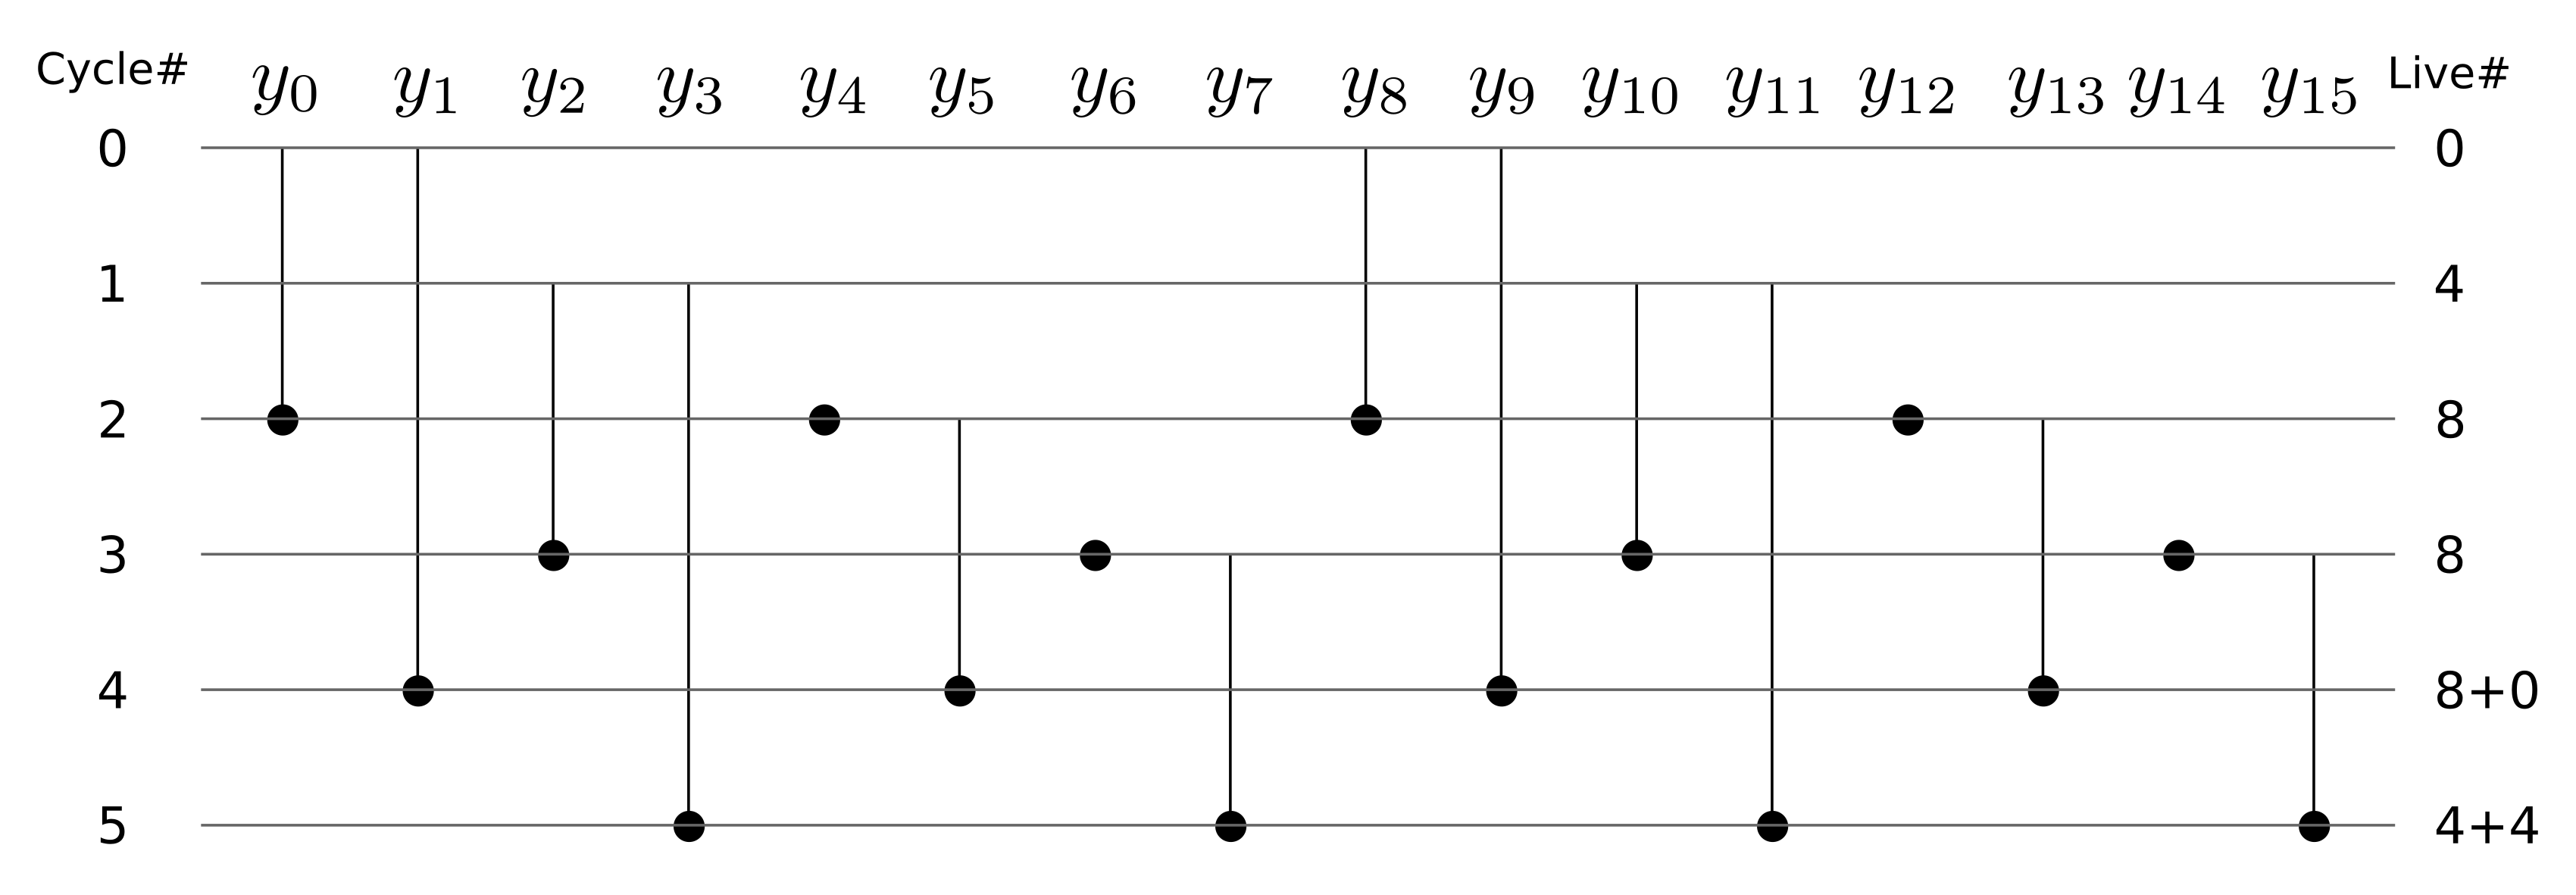
\includegraphics[width=1\linewidth]{Diagramas/life_chart_a.png}%
\caption{Register allocation table for the data represented in \ref{fig:tab-life-a}}
\label{fig:tab-aloc-a}
\end{figure}

\begin{figure}[htbp]%[ht!]
\centering
 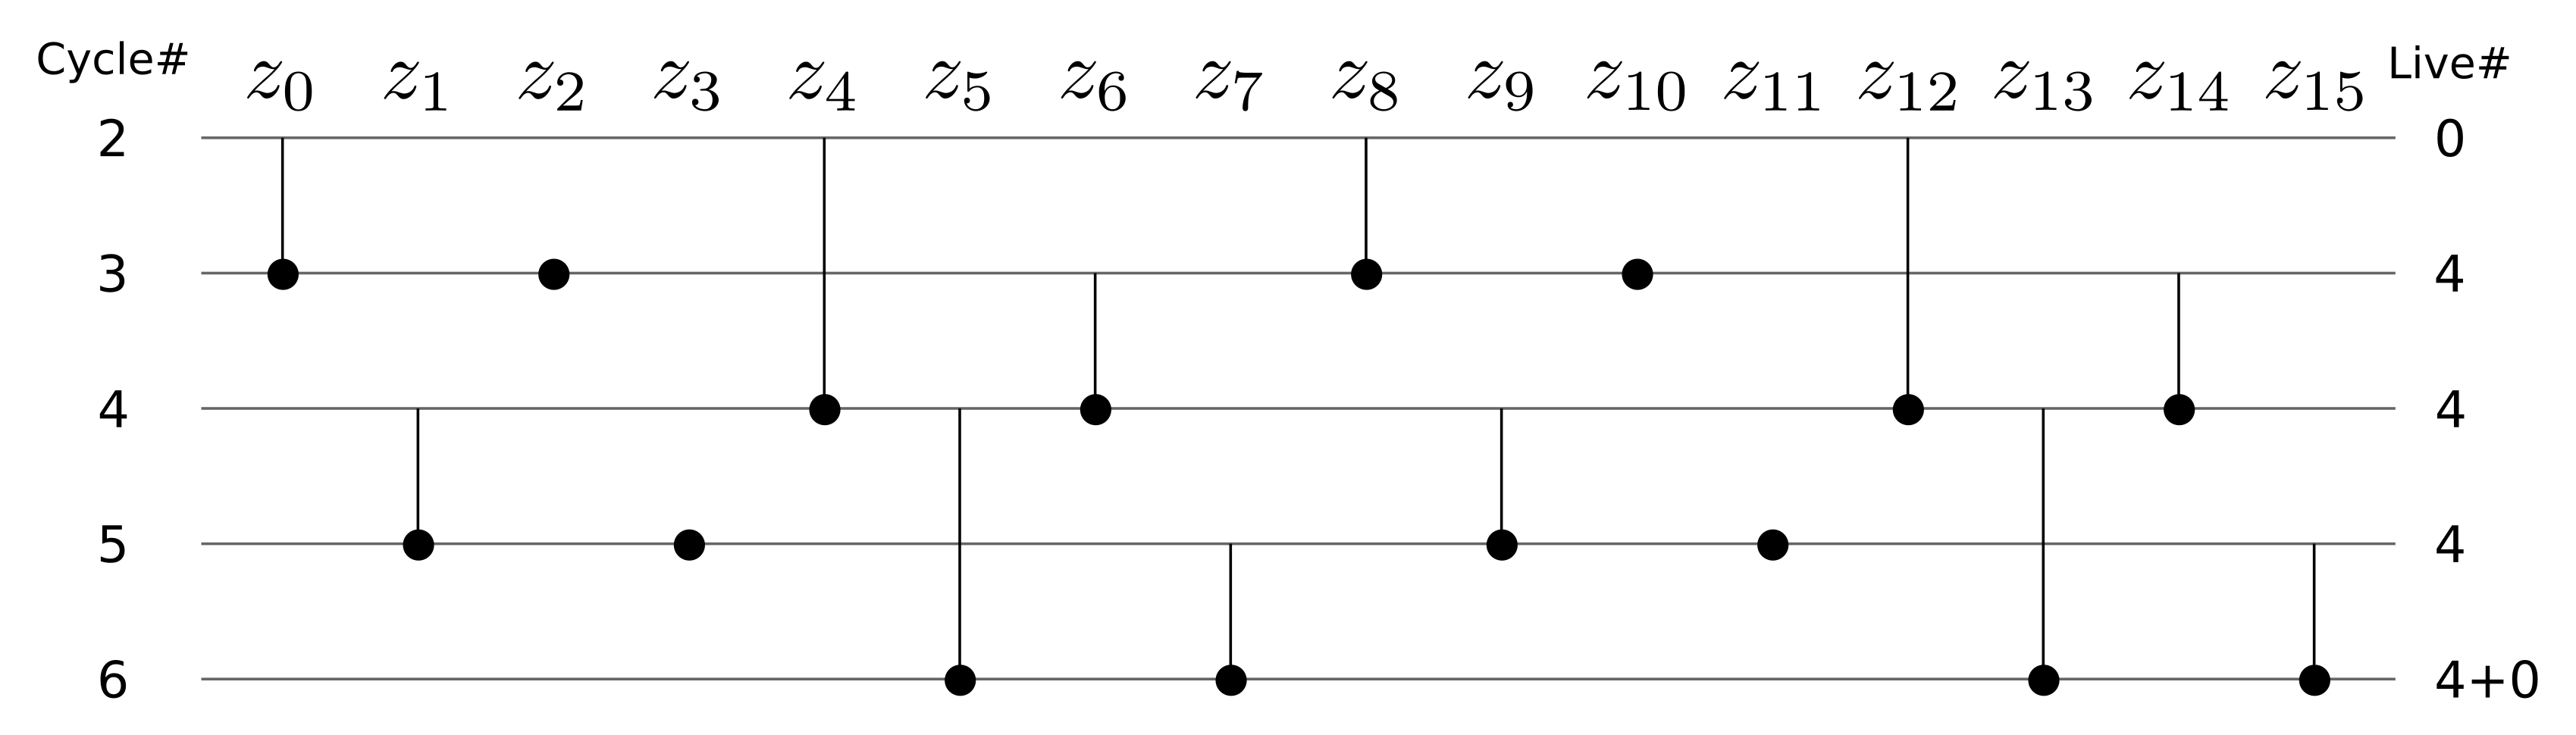
\includegraphics[width=1\linewidth]{Diagramas/life_chart_b.png}%
\caption{Register allocation table for the data represented in \ref{fig:tab-life-b}}
\label{fig:tab-aloc-b}
\end{figure}

\begin{figure}[htbp]%[ht!]
\centering
 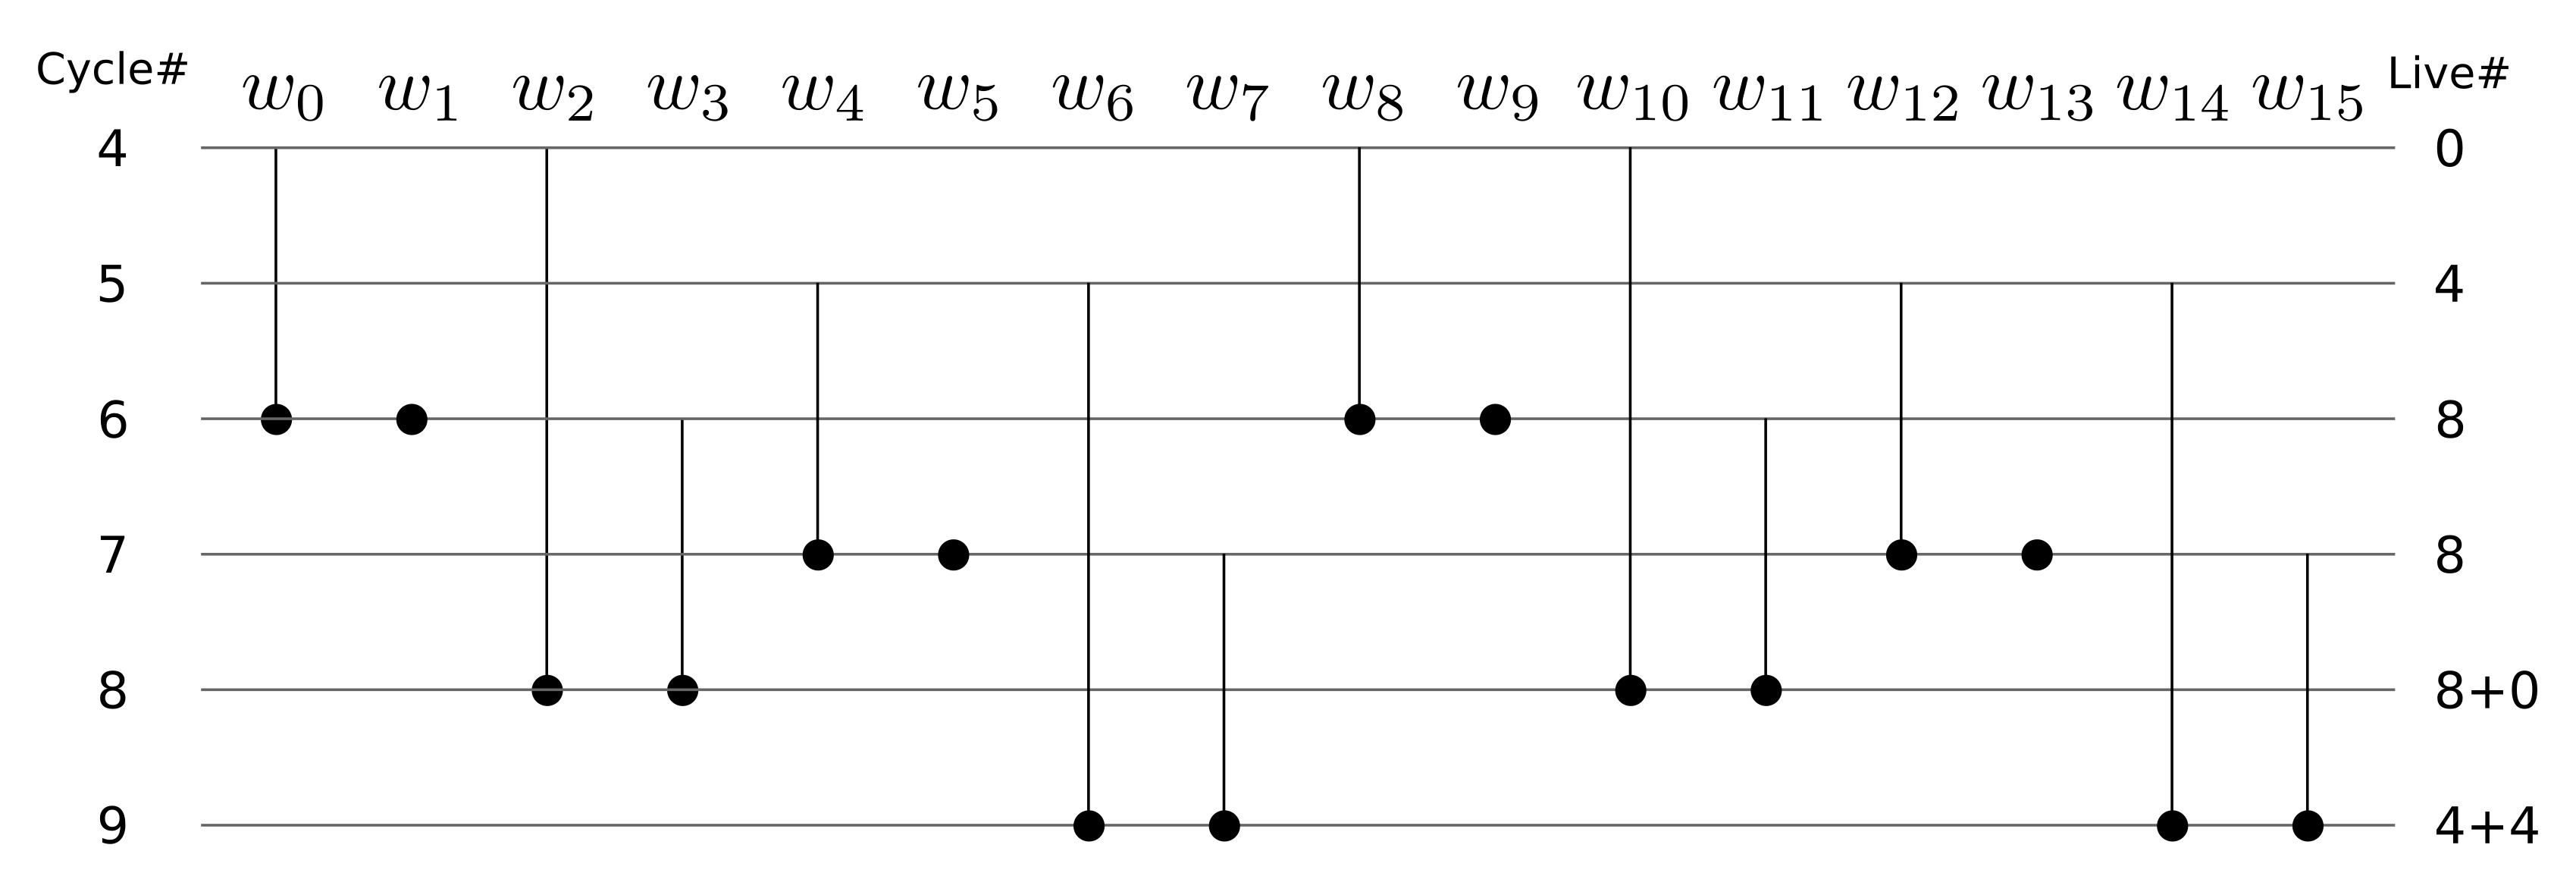
\includegraphics[width=1\linewidth]{Diagramas/life_chart_c.png}%
\caption{Register allocation table for the data represented in \ref{fig:tab-life-c}}
\label{fig:tab-aloc-c}
\end{figure}

\begin{figure*}[htbp]%[ht!]
\centering
 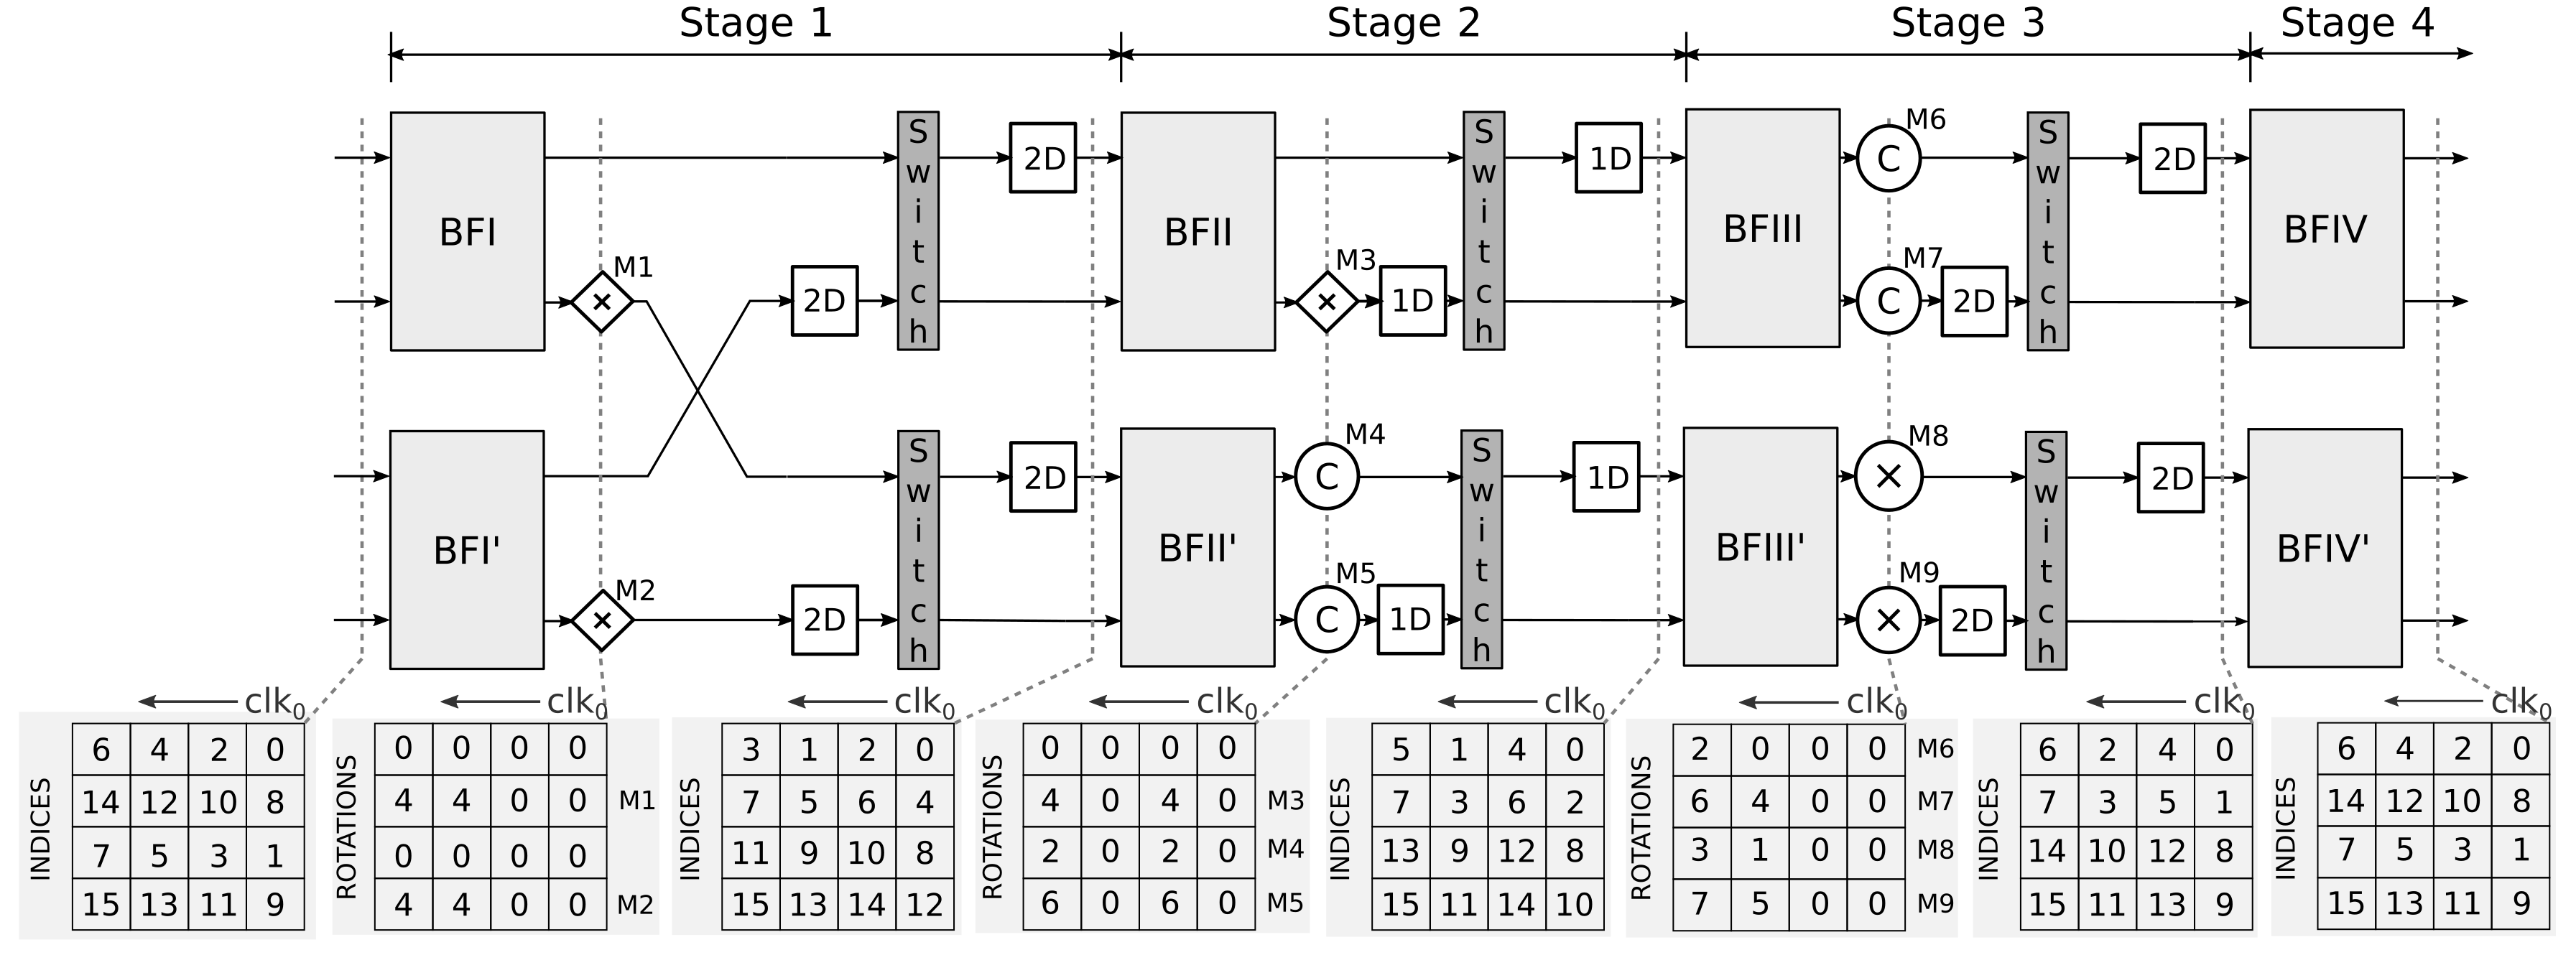
\includegraphics[width=0.85\linewidth]{Diagramas/folding-16.png}%
\caption{Folding architecture for the computation of a radix-$2^3$ 16-point DIF complex FFT.}
\label{fig:circ-folding-16}
\end{figure*}

\begin{figure}[htbp]%[ht!]
\centering
 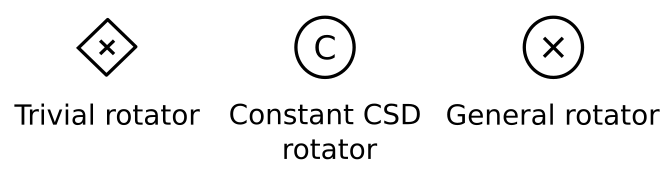
\includegraphics[width=0.85\linewidth]{Diagramas/rotators.png}%
\caption{Symbols used for the different types of rotators}
\label{fig:rotators}
\end{figure}

%%%%%%%%%%%%
% Subseccion
%%%%%%%%%%%%
\subsection{4-Parallel radix-$2^3$ 128-Points}
We can deduce the folding architecture following the same method than used with the 4-Parallel radix-$2^3$ 16-Points. The DFG and folding set used can be shown in Fig. \ref{fig:pipe_dfg_128} and Fig. \ref{tab:fold_set_128} in \ref{sec:appen:pipe_dfg_128} and \ref{sec:appen:folding_set_128}.

The architecture can be seen in Fig. \ref{fig:circ-folding-128}

\begin{figure*}[htbp]%[ht!]
\centering
 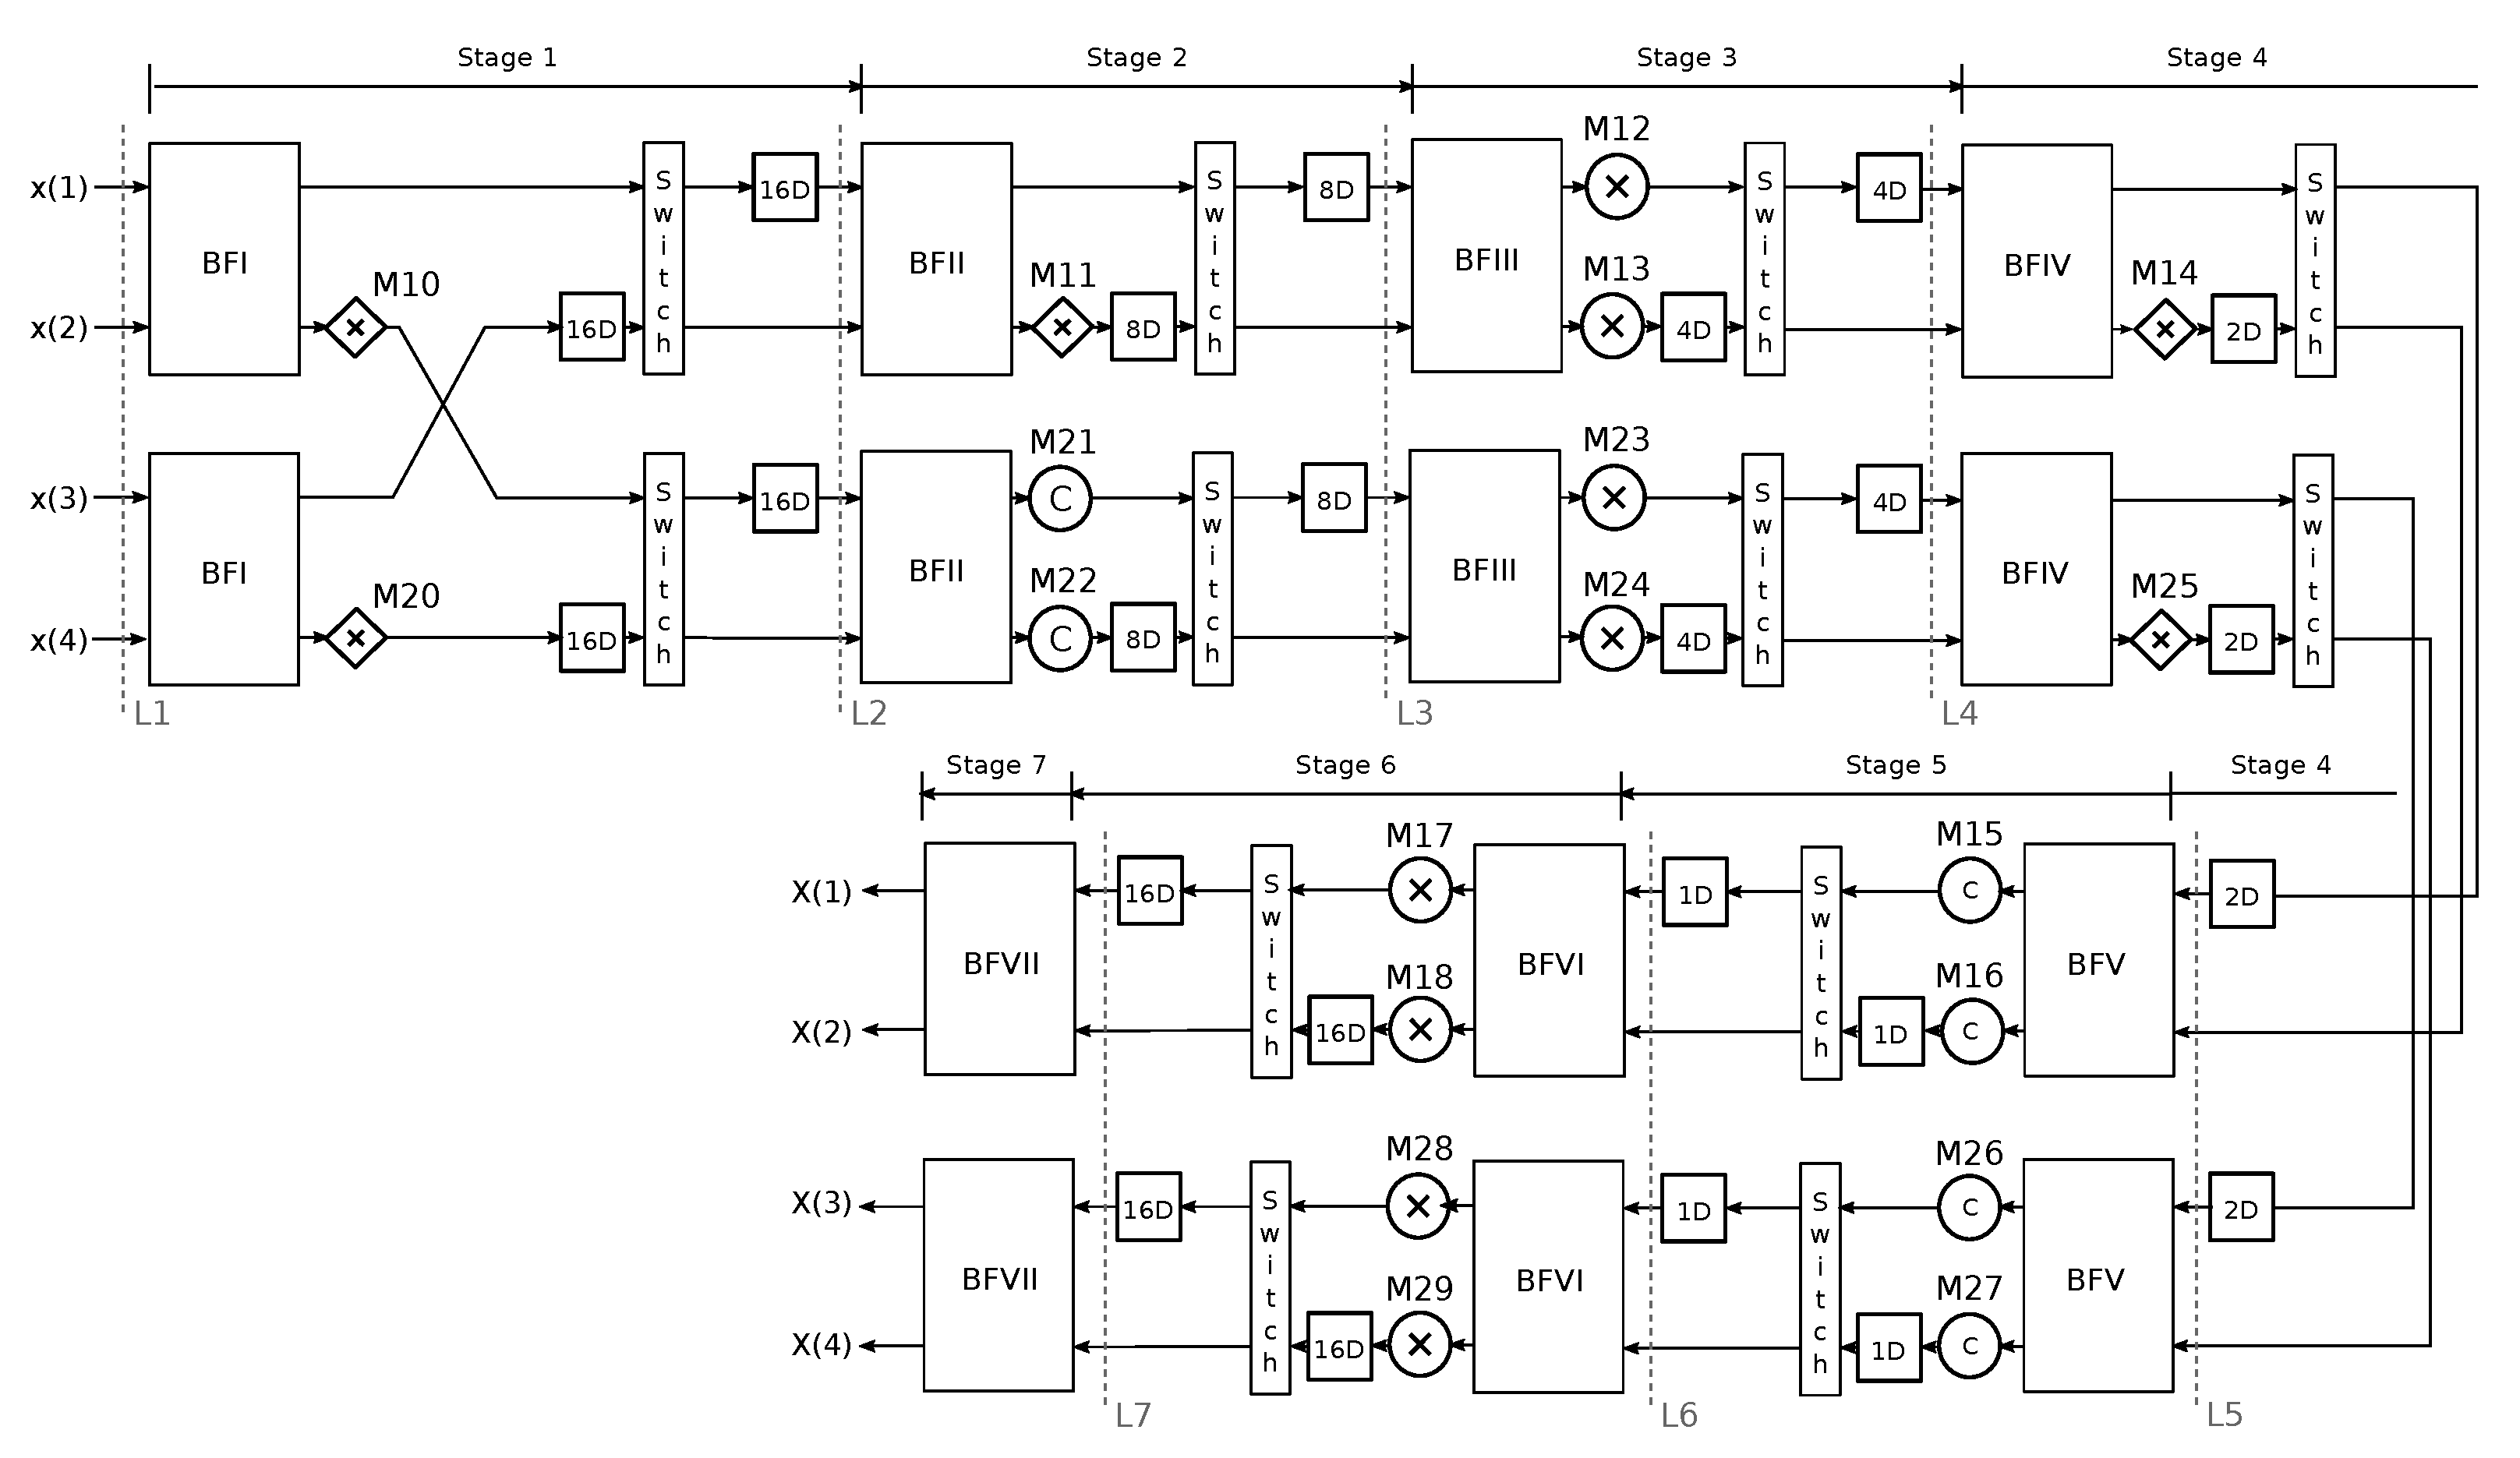
\includegraphics[width=0.95\linewidth]{Diagramas/folding-128.eps}%
\caption{Folding architecture for the computation of a radix-$2^3$ 128-point DIF complex FFT.}
\label{fig:circ-folding-128}
\end{figure*}


%%%%%%%%%
% Seccion
%%%%%%%%%
\section{IMPLEMENTATION}
%%%%%%%%%
% Seccion
%%%%%%%%%
\section{CONCLUSION}
%%%%%%%%%%
% Apendice
%%%%%%%%%%
\section*{APPENDIX}
%%%%%%%%%%%%
% Subseccion
%%%%%%%%%%%%
\subsection{Folding equations for 16-points FFT}
%%%%%%%%%%%%
% Subseccion
%%%%%%%%%%%%
\subsubsection{Without retimming\label{sec:appen:folding_eq}}
\begin{small}
\begin{align*}\small
D_F(D0\to B0)&=2 &  D_F(D0\to B4)&=2\\
D_F(D1\to B1)&=0 &  D_F(D1\to B5)&=0\\
D_F(D2\to B2)&=2 &  D_F(D2\to B6)&=2\\
D_F(D3\to B3)&=-1& D_F(D3\to B7)&=-1\\
D_F(D4\to B0)&=0 &  D_F(D4\to B4)&=0\\
D_F(D5\to B1)&=-1& D_F(D5\to B5)&=-1\\
D_F(D6\to B2)&=0 &  D_F(D6\to B6)&=0\\
D_F(D7\to B3)&=-2& D_F(D7\to B7)&=-2\\
D_F(E0\to C0)&=1 &  D_F(E0\to C2)&=-2\\
D_F(E1\to C1)&=1 &  D_F(E1\to C3)&=2\\
D_F(E2\to C0)&=0 &  D_F(E2\to C2)&=-3\\
D_F(E3\to C1)&=0 &  D_F(E3\to C3)&=1\\
D_F(E4\to C4)&=1 &  D_F(E4\to C6)&=-2\\
D_F(E5\to C5)&=1 &  D_F(E5\to C7)&=2\\
D_F(E6\to C4)&=0 &  D_F(E6\to C6)&=-3\\
D_F(E7\to C5)&=0 &  D_F(E7\to C7)&=1\\
D_F(F0\to D0)&=-2& D_F(F0\to D1)&=0\\
D_F(F1\to D0)&=0 &  D_F(F1\to D1)&=2\\
D_F(F2\to D2)&=2 &  D_F(F2\to D3)&=0\\
D_F(F3\to D2)&=0 &  D_F(F3\to D3)&=-2\\
D_F(F4\to D4)&=-2&  D_F(F4\to D5)&=0\\
D_F(F5\to D4)&=0 &  D_F(F5\to D5)&=2\\
D_F(F6\to D6)&=2 &  D_F(F6\to D7)&=0\\
D_F(F7\to D6)&=0 &  D_F(F7\to D7)&=-2\\
\end{align*}
\end{small}

%%%%%%%%%%%%
% Subseccion
%%%%%%%%%%%%
\subsubsection{With retimming\label{sec:appen:folding_eq_ret}}
\begin{small}
\begin{align*}
D_F(D0\to B0)&=2 &  D_F(D0\to B4)&=2\\
D_F(D1\to B1)&=4 &  D_F(D1\to B5)&=4\\
D_F(D2\to B2)&=2 &  D_F(D2\to B6)&=2\\
D_F(D3\to B3)&=3 &  D_F(D3\to B7)&=3\\
D_F(D4\to B0)&=0 &  D_F(D4\to B4)&=0\\
D_F(D5\to B1)&=3 &  D_F(D5\to B5)&=3\\
D_F(D6\to B2)&=0 &  D_F(D6\to B6)&=0\\
D_F(D7\to B3)&=2 &  D_F(D7\to B7)&=2\\
D_F(E0\to C0)&=1 &  D_F(E0\to C2)&=2\\
D_F(E1\to C1)&=1 &  D_F(E1\to C3)&=2\\
D_F(E2\to C0)&=0 &  D_F(E2\to C2)&=1\\
D_F(E3\to C1)&=0 &  D_F(E3\to C3)&=1\\
D_F(E4\to C4)&=1 &  D_F(E4\to C6)&=2\\
D_F(E5\to C5)&=1 &  D_F(E5\to C7)&=2\\
D_F(E6\to C4)&=0 &  D_F(E6\to C6)&=1\\
D_F(E7\to C5)&=0 &  D_F(E7\to C7)&=1\\
D_F(F0\to D0)&=2 &  D_F(F0\to D1)&=4\\
D_F(F1\to D0)&=0 &  D_F(F1\to D1)&=2\\
D_F(F2\to D2)&=2 &  D_F(F2\to D3)&=4\\
D_F(F3\to D2)&=0 &  D_F(F3\to D3)&=2\\
D_F(F4\to D4)&=2 &  D_F(F4\to D5)&=4\\
D_F(F5\to D4)&=0 &  D_F(F5\to D5)&=2\\
D_F(F6\to D6)&=2 &  D_F(F6\to D7)&=4\\
D_F(F7\to D6)&=0 &  D_F(F7\to D7)&=2\\
\end{align*}
\end{small}

%%%%%%%%%%%%
% Subseccion
%%%%%%%%%%%%
\subsection{Folding set used in 4-parallel  radix-$2^3$ 128-points\label{sec:appen:folding_set_128}}
\begin{table*}[htbp]
\centering
\begin{threeparttable}
\centering
\begin{tabular}{|c||cccccccccccccccc|}
 \hline

  \multirow{2}{*}{A} & A0 & A2 & A4 & A6 & A8 & A10 & A12 & A14 & A16 & A18 & A20 & A22 & A24 & A26 & A28 & A30 \\  

   & A32 & A34 & A36 & A38 & A40 & A42 & A44 & A46 & A48 & A50 & A52 & A54 & A56 & A58 & A60 & A62 \\  
\hline
  \multirow{2}{*}{A'} & A1 & A3 & A5 & A7 & A9 & A11 & A13 & A15 & A17 & A19 & A21 & A23 & A25 & A27 & A29 & A31 \\  

   & A33 & A35 & A37 & A39 & A41 & A43 & A45 & A47 & A49 & A51 & A53 & A55 & A57 & A59 & A61 & A63 \\  
\hline
  \multirow{2}{*}{B} & B1 & B3 & B5 & B7 & B9 & B11 & B13 & B15 & B17 & B19 & B21 & B23 & B25 & B27 & B29 & B31 \\  

   & B0 & B2 & B4 & B6 & B8 & B10 & B12 & B14 & B16 & B18 & B20 & B22 & B24 & B26 & B28 & B30 \\  
\hline
  \multirow{2}{*}{B'} & B33 & B35 & B37 & B39 & B41 & B43 & B45 & B47 & B49 & B51 & B53 & B55 & B57 & B59 & B61 & B63 \\  

   & B32 & B34 & B36 & B38 & B40 & B42 & B44 & B46 & B48 & B50 & B52 & B54 & B56 & B58 & B60 & B62 \\  
\hline
  \multirow{2}{*}{C} & C16 & C18 & C20 & C22 & C24 & C26 & C28 & C30 & C1 & C3 & C5 & C7 & C9 & C11 & C13 & C15 \\  

   & C17 & C19 & C21 & C23 & C25 & C27 & C29 & C31 & C0 & C2 & C4 & C6 & C8 & C10 & C12 & C14 \\  
\hline
  \multirow{2}{*}{C'} & C48 & C50 & C52 & C54 & C56 & C58 & C60 & C62 & C33 & C35 & C37 & C39 & C41 & C43 & C45 & C47 \\  

   & C49 & C51 & C53 & C55 & C57 & C59 & C61 & C63 & C32 & C34 & C36 & C38 & C40 & C42 & C44 & C46 \\  
\hline
  \multirow{2}{*}{D} & D8 & D10 & D12 & D14 & D16 & D18 & D20 & D22 & D24 & D26 & D28 & D30 & D1 & D3 & D5 & D7 \\  

   & D9 & D11 & D13 & D15 & D17 & D19 & D21 & D23 & D25 & D27 & D29 & D31 & D0 & D2 & D4 & D6 \\  
\hline
  \multirow{2}{*}{D'} & D40 & D42 & D44 & D46 & D48 & D50 & D52 & D54 & D56 & D58 & D60 & D62 & D33 & D35 & D37 & D39 \\  

   & D41 & D43 & D45 & D47 & D49 & D51 & D53 & D55 & D57 & D59 & D61 & D63 & D32 & D34 & D36 & D38 \\  
\hline
  \multirow{2}{*}{E} & E4 & E6 & E8 & E10 & E12 & E14 & E16 & E18 & E20 & E22 & E24 & E26 & E28 & E30 & E1 & E3 \\  

   & E5 & E7 & E9 & E11 & E13 & E15 & E17 & E19 & E21 & E23 & E25 & E27 & E29 & E31 & E0 & E2 \\  
\hline
  \multirow{2}{*}{E'} & E36 & E38 & E40 & E42 & E44 & E46 & E48 & E50 & E52 & E54 & E56 & E58 & E60 & E62 & E33 & E35 \\  

   & E37 & E39 & E41 & E43 & E45 & E47 & E49 & E51 & E53 & E55 & E57 & E59 & E61 & E63 & E32 & E34 \\  
\hline
  \multirow{2}{*}{F} & F2 & F4 & F6 & F8 & F10 & F12 & F14 & F16 & F18 & F20 & F22 & F24 & F26 & F28 & F30 & F1 \\  

   & F3 & F5 & F7 & F9 & F11 & F13 & F15 & F17 & F19 & F21 & F23 & F25 & F27 & F29 & F31 & F0 \\  
\hline
  \multirow{2}{*}{F'} & F34 & F36 & F38 & F40 & F42 & F44 & F46 & F48 & F50 & F52 & F54 & F56 & F58 & F60 & F62 & F33 \\  

   & F35 & F37 & F39 & F41 & F43 & F45 & F47 & F49 & F51 & F53 & F55 & F57 & F59 & F61 & F63 & F32 \\  
\hline
  \multirow{2}{*}{G} & G3 & G5 & G7 & G9 & G11 & G13 & G15 & G17 & G19 & G21 & G23 & G25 & G27 & G29 & G31 & G0 \\  

   & G2 & G4 & G6 & G8 & G10 & G12 & G14 & G16 & G18 & G20 & G22 & G24 & G26 & G28 & G30 & G1 \\  
\hline
  \multirow{2}{*}{G'} & G35 & G37 & G39 & G41 & G43 & G45 & G47 & G49 & G51 & G53 & G55 & G57 & G59 & G61 & G63 & G32 \\  

   & G34 & G36 & G38 & G40 & G42 & G44 & G46 & G48 & G50 & G52 & G54 & G56 & G58 & G60 & G62 & G33 \\
\hline
\end{tabular}
\end{threeparttable}
\caption{Folding set for the DFG showed in Fig. \ref{fig:pipe_dfg_128}}
\label{tab:fold_set_128}
\end{table*}


%%%%%%%%%%%%
% Subseccion
%%%%%%%%%%%%
\subsection{Pipelined DFG of a 128-point DIF FFT\label{sec:appen:pipe_dfg_128}}
%\begin{figure*}[htbp]
%\centering
% \includegraphics[width=\linewidth]{Diagramas/bubble_delays_128.eps}%
%\caption{Pipelined DFG of a 128-point DIF FFT as a preprocessing step for folding.}
%\label{fig:pipe_dfg_128}
%\end{figure*}


%\pagebreak


%\begin{landscape}
% \vspace*{\fill}
\begin{figure*}[htbp]%[ht!]%ht!
\centering
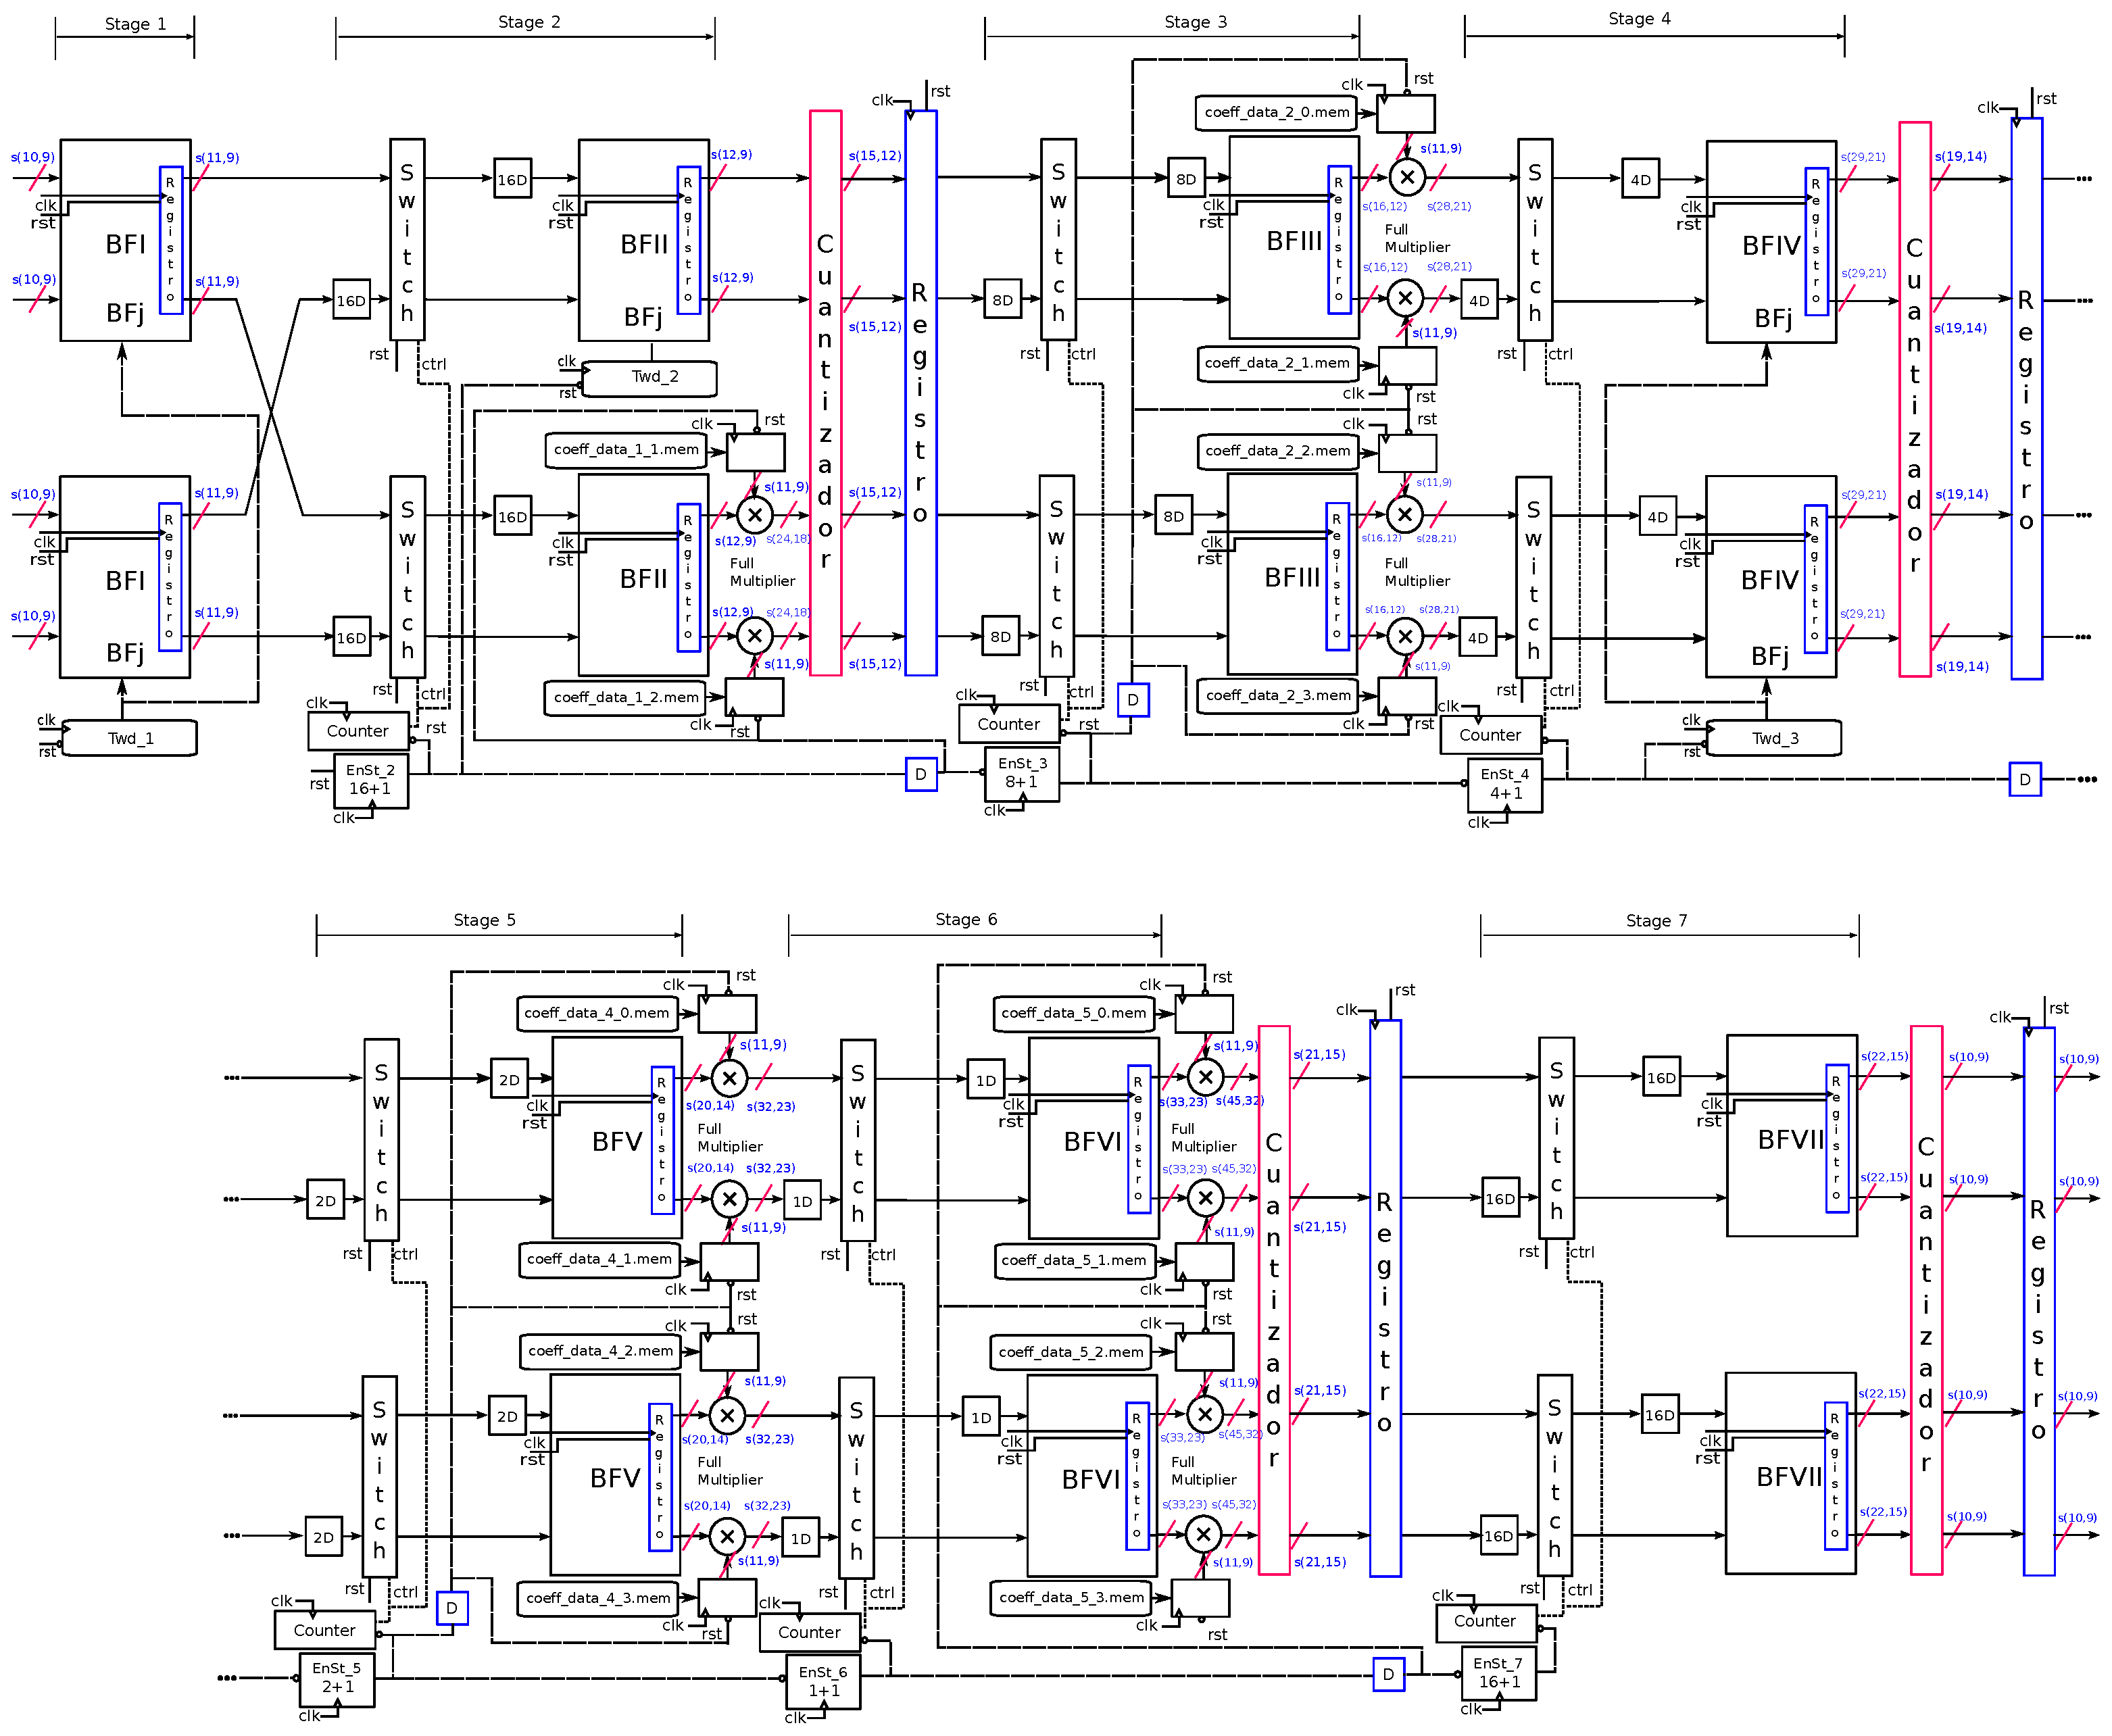
\includegraphics[width=\linewidth]{Diagramas/V5_esquema_p.eps} \\ %
%\label{fig:pipe_dfg_128}
\end{figure*}
 %\vspace*{\fill}
%\end{landscape}


%%%%%%%%%%%%%%
% Bibliografia
%%%%%%%%%%%%%%
\newpage
\bibliographystyle{IEEEtran}
\bibliography{referenciasFFT}
%%%%%%%%
% FIN
%%%%%%%%
\end{document}
